\documentclass[tikz,border=0pt]{standalone}
\usepackage[T1]{fontenc}
\usepackage{lmodern,amsmath,amssymb}
\usetikzlibrary{arrows.meta,calc,positioning}
\definecolor{blue}{HTML}{0072B2}
\definecolor{orange}{HTML}{D55E00}
\definecolor{green}{HTML}{009E73}
\definecolor{ink}{HTML}{25313B}
\renewcommand{\familydefault}{\sfdefault}
\begin{document}
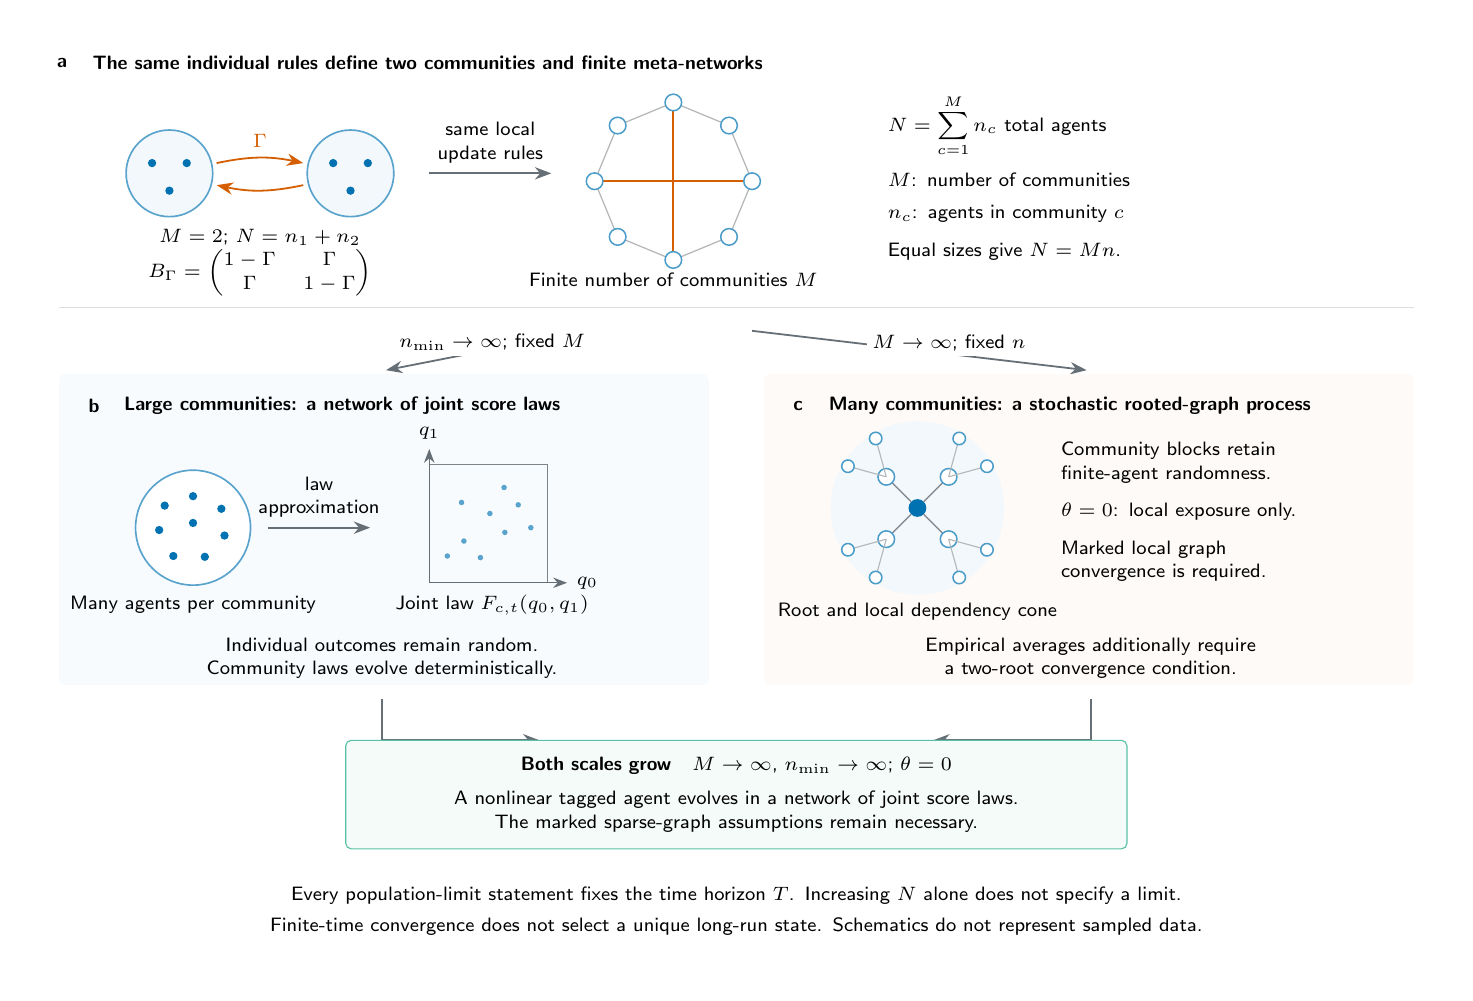
\begin{tikzpicture}[x=1cm,y=1cm,font=\sffamily\fontsize{7}{8.5}\selectfont,>=Stealth,
 arr/.style={->,draw=ink!70,line width=.65pt},
 dot/.style={circle,fill=blue,inner sep=0pt,minimum size=3pt},
 root/.style={circle,fill=blue,draw=blue,inner sep=0pt,minimum size=6pt},
 node/.style={circle,fill=white,draw=blue!70,line width=.55pt,inner sep=0pt,minimum size=6pt},
 note/.style={align=center,text width=7.4cm,inner sep=0pt},
 head/.style={font=\sffamily\fontsize{7}{8.5}\selectfont\bfseries,anchor=west},
 letter/.style={font=\sffamily\fontsize{7}{8.5}\selectfont\bfseries,anchor=west}]
 \path[use as bounding box] (0,0) rectangle (18,12);
 \node[letter] at (.25,11.55) {a};
 \node[head] at (.7,11.55) {The same individual rules define two communities and finite meta-networks};
 \foreach \x/\c in {1.8/A,4.1/B}{
  \draw[blue!65,fill=blue!5,line width=.6pt] (\x,10.15) circle (.55);
  \foreach \dx/\dy in {-.22/.13,.22/.13,0/-.22}{\node[dot] at (\x+\dx,10.15+\dy) {};}
 }
 \draw[arr,orange] (2.4,10.28) to[bend left=12] node[above] {$\Gamma$} (3.5,10.28);
 \draw[arr,orange] (3.5,10.0) to[bend left=12] (2.4,10.0);
 \node[align=center] at (2.95,9.34) {$M=2$; $N=n_1+n_2$};
 \node[align=center] at (2.95,8.89) {$\displaystyle B_\Gamma=\begin{pmatrix}1-\Gamma&\Gamma\\\Gamma&1-\Gamma\end{pmatrix}$};
 \draw[arr] (5.1,10.15)--node[above,align=center] {same local\\update rules} (6.65,10.15);
 \foreach \i in {0,...,7}{\coordinate (v\i) at ($(8.2,10.05)+(45*\i:1.0)$);}
 \foreach \i in {0,...,7}{
  \pgfmathtruncatemacro{\j}{mod(\i+1,8)}
  \draw[ink!35,line width=.45pt] (v\i)--(v\j);
 }
 \draw[orange,line width=.7pt] (v0)--(v4) (v2)--(v6);
 \foreach \i in {0,...,7}{\node[node] at (v\i) {};}
 \node[align=center] at (8.2,8.8) {Finite number of communities $M$};
 \node[align=left,text width=5.7cm,anchor=west] at (10.8,10.1) {$\displaystyle N=\sum_{c=1}^{M}n_c$ total agents\\[5pt]$M$: number of communities\\[3pt]$n_c$: agents in community $c$\\[5pt]Equal sizes give $N=Mn$.};
 \draw[ink!16,line width=.5pt] (.4,8.45)--(17.6,8.45);
 \draw[arr] (7.1,8.15)--(4.55,7.65);
 \node[fill=white,inner sep=2pt] at (5.9,8.0) {$n_{\min}\to\infty$; fixed $M$};
 \draw[arr] (9.2,8.15)--(13.45,7.65);
 \node[fill=white,inner sep=2pt] at (11.7,8.0) {$M\to\infty$; fixed $n$};
 \fill[blue!3,rounded corners=2pt] (.4,3.65) rectangle (8.65,7.6);
 \fill[orange!3,rounded corners=2pt] (9.35,3.65) rectangle (17.6,7.6);
 \node[letter] at (.65,7.2) {b};
 \node[head] at (1.1,7.2) {Large communities: a network of joint score laws};
 \draw[blue!65,fill=white,line width=.6pt] (2.1,5.65) circle (.73);
 \foreach \dx/\dy in {-.36/.28,0/.4,.36/.24,-.43/-.03,0/.06,.4/-.1,-.25/-.36,.15/-.37}{\node[dot] at (2.1+\dx,5.65+\dy) {};}
 \node at (2.1,4.67) {Many agents per community};
 \draw[arr] (3.05,5.65)--node[above,align=center] {law\\approximation} (4.35,5.65);
 \draw[ink!60,line width=.5pt] (5.1,4.95) rectangle (6.6,6.45);
 \draw[arr,line width=.45pt] (5.1,4.95)--(6.85,4.95) node[right] {$q_0$};
 \draw[arr,line width=.45pt] (5.1,4.95)--(5.1,6.65) node[above] {$q_1$};
 \foreach \dx/\dy in {.23/.34,.44/.53,.41/1.02,.65/.32,.77/.88,.96/.64,1.13/.99,.95/1.21,1.29/.7}{\fill[blue!65] (5.1+\dx,4.95+\dy) circle (.035);}
 \node at (5.9,4.67) {Joint law $F_{c,t}(q_0,q_1)$};
 \node[note] at (4.5,3.99) {Individual outcomes remain random.\\Community laws evolve deterministically.};
 \node[letter] at (9.6,7.2) {c};
 \node[head] at (10.05,7.2) {Many communities: a stochastic rooted-graph process};
 \fill[blue!5] (11.3,5.9) circle (1.1);
 \node[root] (o) at (11.3,5.9) {};
 \foreach \i in {0,...,3}{
  \coordinate (u\i) at ($(11.3,5.9)+(45+90*\i:.56)$);
  \draw[ink!55,line width=.5pt] (o)--(u\i);
  \node[node] at (u\i) {};
  \foreach \j in {-14,14}{
   \coordinate (w) at ($(11.3,5.9)+(45+90*\i+\j:1.03)$);
   \draw[ink!35,line width=.4pt] (u\i)--(w);\node[node,minimum size=4.5pt] at (w) {};
  }
 }
 \node[align=center] at (11.3,4.58) {Root and local dependency cone};
 \node[align=left,text width=3.8cm,anchor=west] at (13.0,5.85) {Community blocks retain\\finite-agent randomness.\\[5pt]$\theta=0$: local exposure only.\\[5pt]Marked local graph\\convergence is required.};
 \node[note] at (13.5,3.99) {Empirical averages additionally require\\a two-root convergence condition.};
 \draw[arr] (4.5,3.48)--(4.5,2.95)--(6.5,2.95);
 \draw[arr] (13.5,3.48)--(13.5,2.95)--(11.5,2.95);
 \node[draw=green!65,fill=green!4,rounded corners=2pt,align=center,text width=9.5cm,inner sep=6pt] at (9,2.26) {\textbf{Both scales grow}\quad\mbox{$M\to\infty$, $n_{\min}\to\infty$; $\theta=0$}\\[4pt]A nonlinear tagged agent evolves in a network of joint score laws.\\The marked sparse-graph assumptions remain necessary.};
 \node[align=center,text width=16.7cm] at (9,.78) {Every population-limit statement fixes the time horizon $T$. Increasing $N$ alone does not specify a limit.\\[3pt]Finite-time convergence does not select a unique long-run state. Schematics do not represent sampled data.};
\end{tikzpicture}
\end{document}
